% easychair.tex,v 3.1 2011/12/30
%
% Select appropriate paper format in your document class as
% instructed by your conference organizers. Only withtimes
% and notimes can be used in proceedings created by EasyChair
%
% The available formats are 'letterpaper' and 'a4paper' with
% the former being the default if omitted as in the example
% below.
%
\documentclass[procedia]{easychair}
%\documentclass[debug]{easychair}
%\documentclass[verbose]{easychair}
%\documentclass[notimes]{easychair}
%\documentclass[withtimes]{easychair}
%\documentclass[a4paper]{easychair}
%\documentclass[letterpaper]{easychair}

% This provides the \BibTeX macro
\usepackage{doc}
\usepackage{makeidx}
\usepackage{multirow}
\usepackage{array}

% In order to save space or manage large tables or figures in a
% landcape-like text, you can use the rotating and pdflscape
% packages. Uncomment the desired from the below.
%
% \usepackage{rotating}
% \usepackage{pdflscape}

% If you plan on including some algorithm specification, we recommend
% the below package. Read more details on the custom options of the
% package documentation.
%
% \usepackage{algorithm2e}

% Some of our commands for this guide.
%
\newcommand{\easychair}{\textsf{gpnn}}
\newcommand{\miktex}{MiK{\TeX}}
\newcommand{\texniccenter}{{\TeX}nicCenter}
\newcommand{\makefile}{\texttt{Makefile}}
\newcommand{\latexeditor}{LEd}

\def\procediaConference{99th Conference on Topics of
  Superb Significance (COOL 2014)}

%\makeindex

%% Front Matter
%%
% Regular title as in the article class.
%
\title{A Computational Framework for Implementation of\\
       Neural Networks on Multicore Machine}

% \titlerunning{} has to be set to either the main title or its shorter
% version for the running heads. When processed by
% EasyChair, this command is mandatory: a document without \titlerunning
% will be rejected by EasyChair

\titlerunning{Parallelized Neural Networks Framework}

% Authors are joined by \and. Their affiliations are given by \inst, which indexes into the list
% defined using \institute
%
\author{
    Wenduo Wang\inst{1}%\thanks{Designed and implemented the class style}
\and
    Yi L. Murphey\inst{2}%\thanks{Masterminded EasyChair and created versions 3.0--3.4 of the class style}\\
}

% Institutes for affiliations are also joined by \and,
\institute{
  University of Michigan-Dearborn,
  Dearborn, Michigan, U.S.A\\
  \email{wenduow@umich.edu}
\and
   University of Michigan-Dearborn,
   Dearborn, Michigan, U.S.A\\
   \email{yilu@umich.edu}\\
}

%  \authorrunning{} has to be set for the shorter version of the authors' names;
% otherwise a warning will be rendered in the running heads. When processed by
% EasyChair, this command is mandatory: a document without \authorrunning
% will be rejected by EasyChair

\authorrunning{Wang and Murphey}

\begin{document}

\maketitle

\keywords{algorithm, back-propagation, neural networks, parallel computing, generic programming}

\begin{abstract}

This paper presents a computational framework, GPNN, for efficient implementation of Back-Propagation based neural network training on multithread and multicore machines. GPNN has three components, parallelization of training process, abstraction modeling of network components, and generic programming to make neural network systems to change architectural configurations.  The penalization component distributes training data to multicores to calculate errors, which are then summarized and used for weight update based on gradient descent the multithread programming to take advantage of a multicore computer architecture.  The abstraction component models input, bias, weight, and neuron all as nodes, which make the training process in a parallel computer architecture much more efficient.  The generic programming component will make a neural network system easy to change its configurations and easily transported among different operating systems or computer hardware systems.  The GPNN was applied to four different neural learning algorithms, Classic Back-Propagation (BP), Quick Propagation (QP), Resilient Propagation (RP) and Levenberg-Marquardt Algorithm (LM), and experiments are conducted to evaluate the efficiency of these neural network algorithms implemented under the GPNN framework.

\end{abstract}

%------------------------------------------------------------------------------

\section{Introduction}

Artificial neural networks are used in wide range of research and applications over past three decades.  The network topology and propagation algorithms often vary with different application scenarios.  Researchers usually spend much effort and time struggling to try different network architectures, applying them to training data, and analyzing training results.  Many important issues, for example, over-fitting, network size, memory space need to be considered across the whole training procedure.  This may shifts researchers from their original topics to too much network reliability considerations.

Benefited from generic programming, researchers can easily configure their own neural networks or try among different configurations through a design pattern, as known as the policy pattern, which makes everything instantiable modules.  This library currently provides four types of networks, which are 1, 2, 3-hidden layer networks and recurrent network \cite{boden2001guide}, four types of weight update algorithms, classic back-propagation (BP), quick propagation (QP) \cite{fahlman1988empirical}, resilient propagation (RP) \cite{riedmiller1993direct} and Levenberg-Marquardt algorithms (LM) \cite{hagan1994training}.  Besides these build-in learning models, researchers can connect or prune perceptron (using neuron instead of perceptron in rest of the article for convenience) and weights to customize any type of network topology.

With the increase number of cores or processors, appropriate parallelization and data partition can maximum training speed.  The GPNN library provides the interface for fast local file access using memory map and an interface for Map-Reduce application.  All of these operations and inner data flows during training are implemented on stack memory to avoid wasting time on dynamic allocation and access.  The only restriction of network size depends on the stack pre-allocation of compiler, which normally can be adjusted by compilers.

Different from previous works, for example, FANN \cite{nissen2003implementation}, OpenNN \cite{lopezopennn} and tnnlib, which take only partial advantages of generic programming, algorithm and topology diversity or parallel execution ability (see Appendix~ref{appendix:comparison}), the GPNN library possesses all of these attractive characteristics.

%------------------------------------------------------------------------------

\section{A Computational Framework for Implementing Neural Learning Algorithms on Multicore machines}

The proposed computational framework consists of three major components, parallelization of training process using a multithread scheme, abstraction of network components, and general programming on transfer functions, error functions and network topologies.  First we present a formal description of neural network structures and back-propagation neural learning algorithm from the perspective of software implementation.

In software implementation development, a classic neural network layer is normally modeled as a container, which holds a weight matrix, a bias node and multiple neurons.  Additionally, it specifies the propagation order of these components.  In a global view, layer can be connected with each other.

Back-Propagation is the most popular neural learning algorithm for supervised learning in multi-layered feed-forward networks as well as in many recurrent neural networks.  Most of the neural networks have a unique forward path.

\begin{gather}
    net_j = \sum_i w_{ji} x_i \notag \\
    x_j = f_j(net_j) \notag
\end{gather}

where $x_i$ is the outputs from the neuron $i$ in previous layer, which is regarded as the inputs of neuron $j$, $w_{ji}$ is the weight from all previous neuron $i$ to neuron $j$, net is calculated as the weighted sum of all the inputs, and $x_j$ is the output after $net_j$ filtered by the transfer function $f_j$, which is also regarded as one of the input of next layer.

The backward path follows gradient descent calculated by chain rule.

\begin{equation}
    \frac{ \partial E_j }{ \partial w_{ji} } = \frac{ \partial E_j }{ \partial x_j } \cdot \frac{ \partial x_j }{ \partial net_j } \cdot \frac{ \partial net_j }{ \partial w_{ji} } = \frac{ \partial E_j }{ \partial x_j } f'_j(net_j) x_i \notag
\end{equation}

For every hidden neuron, its gradient is affected by all of its successors.  To consistently express the gradient of output nodes and hidden nodes, let

\begin{equation}
    \delta_{ji,d} = \left \{
    \begin{array}{l l}
        t_d - y_d & \quad \text{for output neuron} \\
        \sum_k {w_{kj}\delta_{kj,d} } & \quad \text{for hidden neuron}
    \end{array} \right. \notag
\end{equation}

where $k$ contributes to next layer.

\subsection{Parallelization}

According to Moore’s law, the density of circuits doubling at every new generation \cite{chu2007map}.  In the recent years, computer systems have increased number of cores to support parallel computing.  In big data applications, it is important to implement neural learning algorithms in high level of parallelization on multicore CPUs with shared memory to achieve significant increases in CPU performance.  We propose an approach of multithread implementation of batch training BP \cite{schuessler2011parallel}.  The approach is illustrated in \ref{fig:parallelization}, where it is shown in a $K$-thread parallel computing structure, where an neural network is copies $K$ times, and the training data are distributed to these $K$ threads.  The input are processed.

\begin{figure}[tb]
    \begin{centering}
        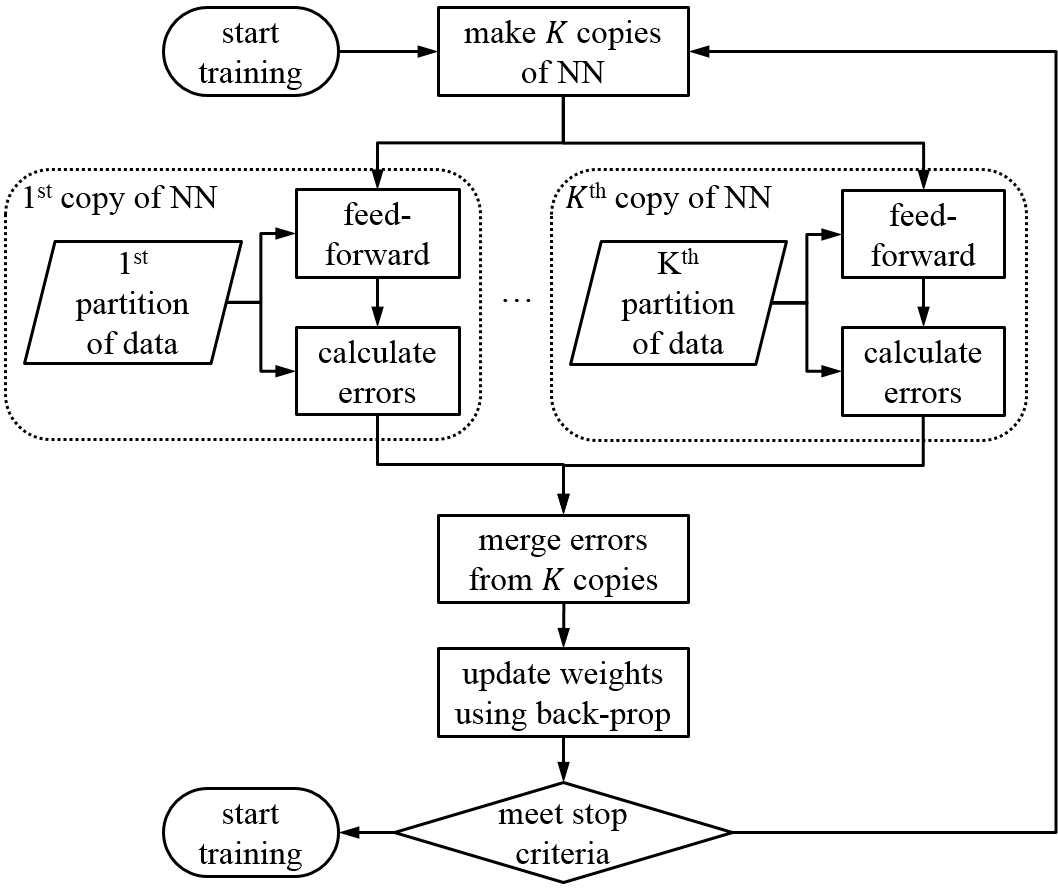
\includegraphics[scale=1]{../../pic/parallelization.png}
        \caption{Multithread training procedure is a modification of traditional batch mode training.  Weights will copy to several network images.  Each image will feed-forward its training patterns and back-propagate gradients.  Gradients of different network images will then merged together to be updated.  The whole runs in a loop until stop criteria is met.}
    \label{fig:parallelization}
	\end{centering}
\end{figure}

Simultaneously along the feed-forward paths of these $K$ threads, and errors are calculated at the end of each thread.  Then the errors at all $K$ threads are combined for weight update using gradient descent (back-propagation path), which is represented as follows,

\begin{equation}
    \frac{\partial E_j}{\partial w_{ji}} = \sum_k \frac{\partial E_j^{(k)}}{\partial w_{ji}^{(k)}} \notag
\end{equation}

Weights are then all updated through back-The updated neural network is made K copies, and the same training process is repeated until user defined stop criteria are satisfied.

\subsection{Abstraction of Weight, Neuron, Bias, Input and Target}

Abstraction is a very critical and powerful concept in object-oriented programming which means to abstract as objects of similar functions to the same module.  Based on this concept, weights between neurons can be considered as similar to neurons, since a neuron has one input axon and one output axon, and a weight connecting two neurons can also be considered to have an input, which is the output axon of the preceding neuron, and the weight can be considered as its output axon that is connected to the input axon of following neuron.  The transfer function of a weight is defined as follows.

\begin{align}
    & \text{feed-forward:} & x_{ji} = f_{ji}(x_i) = w_{ji}x_i \notag \\
    & \text{back-propagation:} & \delta_j = w_{ji}\delta_{ji} \notag
\end{align}

For the same reason, an input node to a neural network can also be treated similar to a neuron, which has the equal number of output axons to the first hidden layer but no input axon.  Similarly, bias of a neuron layer can also be handled in this way.  There is no back-propagation for any of these input nodes.

\begin{align}
	& \text{feed-forward for input:} & x_i = f_0(p) = p \notag \\
	& \text{feed-forward for bias:} & x_b = f_b(1) = 1 \notag
\end{align}

where $p$ is the value of input feature, $x_i$ is the output of the input node, and the output of the bias node $x_b$ is always 1.  [you're here]

Contrarily, a target node can have one input axon connected to the output of a neural network but no output axon.  There is no feed-forward for target node.

\begin{align}
    & \text{back-propagation for output:} & \delta_j = t_j - y_j \notag
\end{align}

where $t_j$ is the target value of this output node, and $y_j$ is the network predicted value.

To sum up above abstraction, input, bias, weight, neuron and target will be aliased as node in following context.  Each kind of node will be grouped by an abstracted layer and these abstracted layer will be connected to each other instead of directly connecting classic layer illustrated in fig.~\ref{fig:nn_classic}.  The connection among nodes and abstracted layer therefore can be equivalently looked upon while programming.

\begin{figure}[tb]
    \begin{centering}
        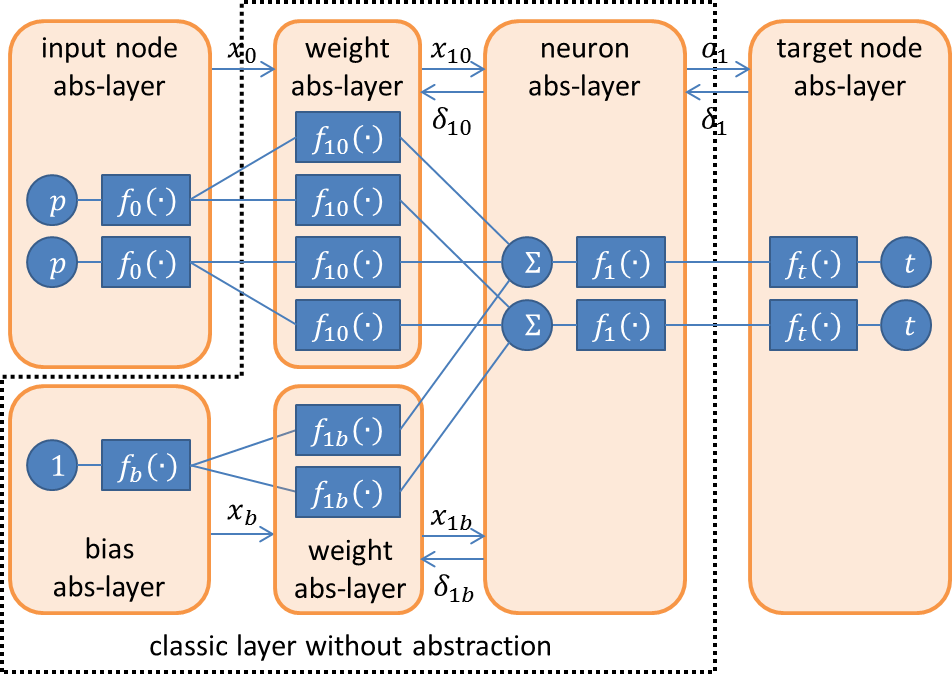
\includegraphics[scale=0.5]{../../pic/nn_abstracted.png}
        \caption{1-layer neural network topology with abstracted layer (abs-layer) interpretation.  The abstracted layers inside the dash-line compose a classic layer.}
        \label{fig:nn_abstracted}
	\end{centering}
\end{figure}

Considering the convenience provided for implementing parallel computing algorithm, only weight abstracted layers need to be copied or shared among network images.  The rest part of the network, such as input nodes, biases, neurons and target nodes, can remain local on distributed systems.  This brings less communicational memory cost, which highly correlated to time consumption in parallelized implementation, will improve multithread efficiency.

Current input and output of a node will be stored for each input pattern in order to provide any convenience in processing weight update algorithm.  Other values are prepared during feed-forward or back-propagation for intermediate calculation of critical variables, for example, $f(net)$ and $f'(net)$.

\begin{figure}[tb]
    \begin{centering}
        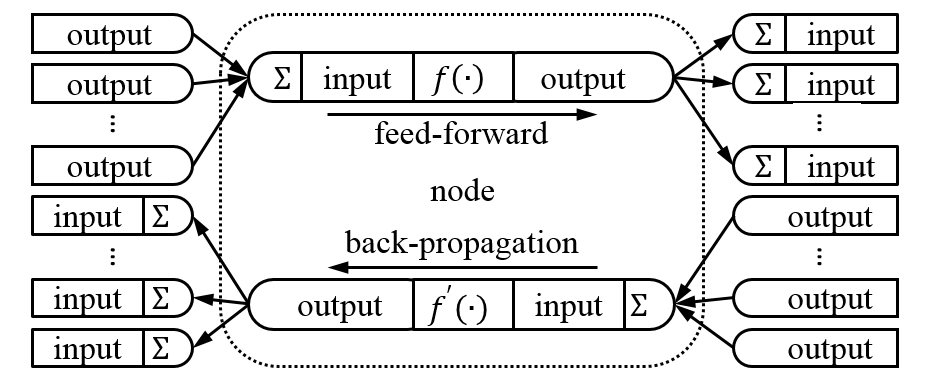
\includegraphics[scale=0.5]{../../pic/microscopic.png}
        \caption{A microscopic view of node.  It connects the outputs and inputs of other nodes.}
        \label{fig:microscopic}
	\end{centering}
\end{figure}

\subsection{Compile-Time Generalization to Learning Algorithms, Transfer Functions, Error Functions and Network Topologies}

Generic programming is one of the best implementation approaches to generalize any type of replaceable functional node in neural networks, in which architecture is written in terms of types to-be-specified-later \cite{wiki:generic_programming} that are then instantiated when needed for specific types provided as parameters.  Thanks to template mechanism in C++, it is a good candidate for coping with combinatorial behavior data types, which refers to neural learning algorithms, transfer functions, network topologies, error functions and other training factors here because behavior data types can be deduced statically during compiling period \cite{alexandrescu2001preface}.  This compile-time generalization technique avoids extra time consumption during each loop to determine the running type of an object through looking up its virtual table, which a run-time generalization usually implements through.  For example, weight will provide forward, backward, update, copy and merge interfaces.  User can easily specify an appropriate update strategy of weight during programming without modifying rest part of the code.  The compiler will compile a made-to-order target file related to developer customized behavior data types.  In addition, since the software is tailored with specific behavior data types at compiling period, it greatly reduces irrelevant code to be compiled, thus, reduces software size.

\begin{figure}[tb]
    \begin{centering}
        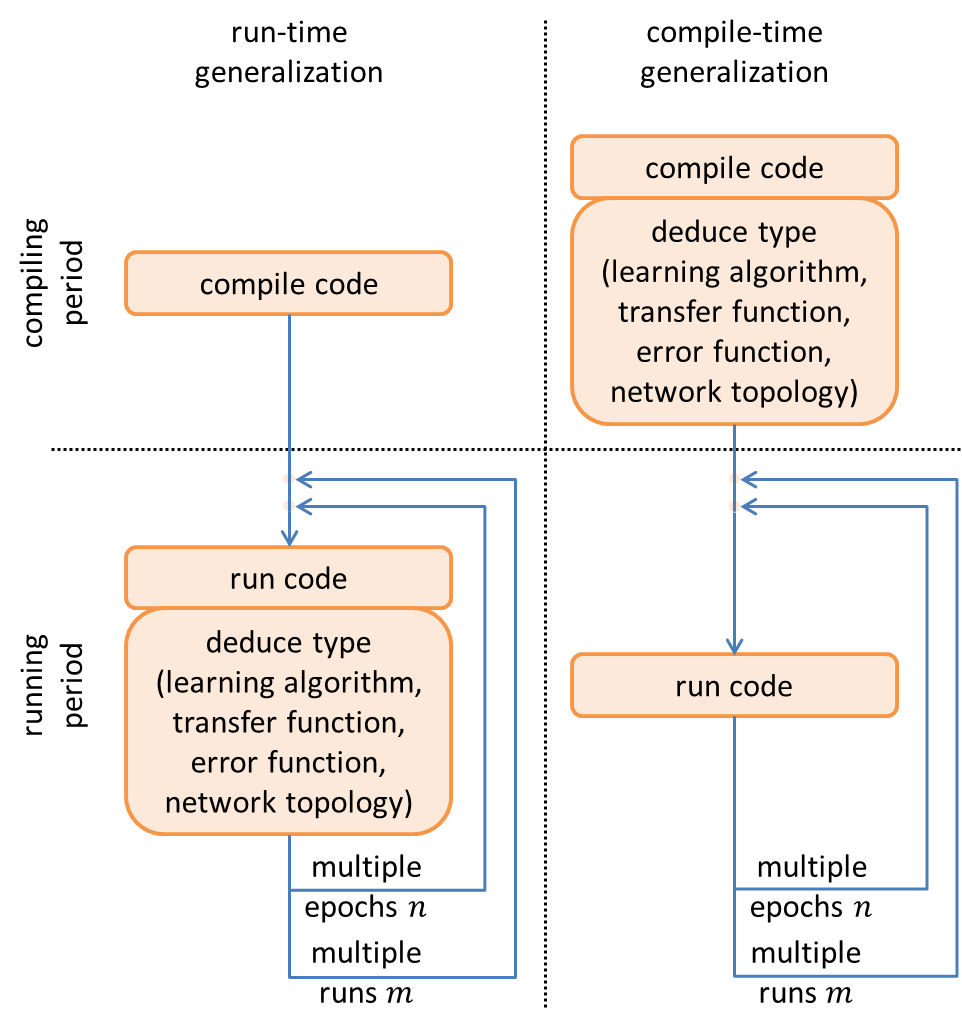
\includegraphics[scale=0.5]{../../pic/run_vs_compile.png}
        \caption{Run-time generalization versus compile-time generalization from compiling code to running code.  $n$ is epoch number and $m$ is experiment running times.}
        \label{fig:run_vs_compile}
	\end{centering}
\end{figure}

As illustrated in above fig.~\ref{fig:run_vs_compile}, weight type will be deduced in every epoch during run-time generalization, which means that the processors spend time on deciding weight type in each loop through looking up virtual table.  As a consequence, the accumulative time consumption from all loops is conspicuous.  However, the compile-time generalization only deduces type onetime at compiling period.  There is no extra time consumption during each loop.  Moreover, if the neural networks software is required to be run multiple times for different experimental purposes, run-time generalization cannot avoid taking time on type deduction during each loop and each run.  Contrarily, because there’s no need to compile the same neural network software again for these experiments, the compile-time generalization could absolutely get rid of running time consumption.  To sum up, the time complexity for run-time generalization is $O(mn)$, but there’s no extra cost while running after compile-time generalization $O(1)$.

In terms of design pattern, this compile-time generalization approach is as known as policy based class design \cite{alexandrescu2001policy}.  In the library implementation, each learning algorithm is defined as a kind of update policy, each transfer function is defined as a kind of transfer policy, each network topology is defined as a kind of topology policy, each error function is defined as a kind of error policy, even the number of neurons, input, target and other training factors can be considered as individual value policies as well.

\subsection{Scalability and Reusability}

Scalability is an important measurement of a software library.  A high scalable software library could provide freedom space for further development or maintenance.  Benefit from abstraction and compile-time generalization, researchers can easily customize their own neural networks by simply connecting or pruning nodes without re-design the most part of the network architecture.  For example, one would like to implement a recurrent neural network without bias using LM algorithm and log-sigmoid transfer function based on an existing biased 1-layer neural network using BP algorithm and linear transfer function.  It is simple to modify following 3 steps.

\begin{enumerate}
    \item Detach a bias abstracted layer and a weight abstracted layer.
    \item Attach a neuron abstracted layer using linear transfer function, and attach a weight abstracted layer using LM algorithm.
    \item Replace the algorithm type of the weight abstracted layer from BP to LM, and replace the transfer function type of the neuron abstracted layer from log-sigmoid to linear.
\end{enumerate}

\begin{figure}[h]
    \begin{centering}
        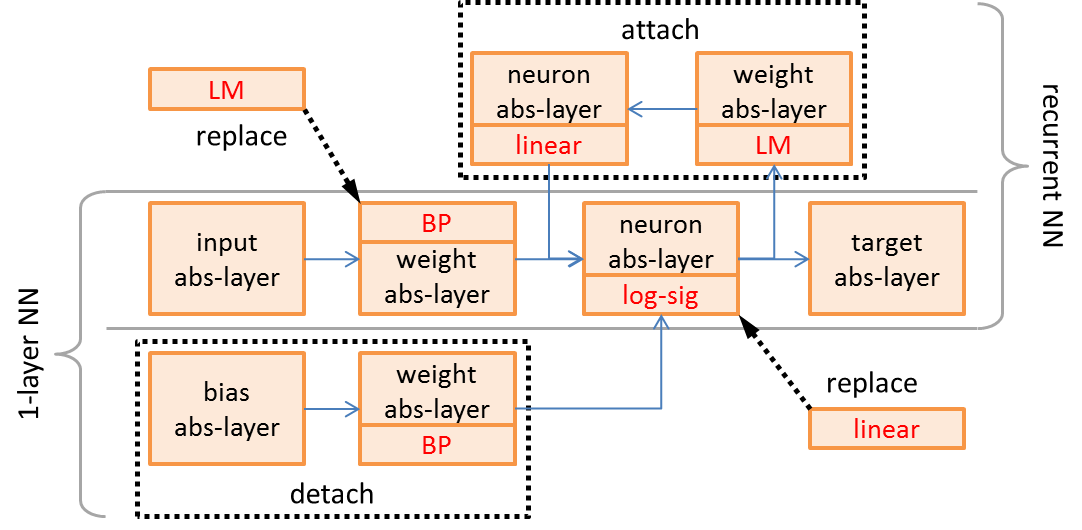
\includegraphics[scale=0.5]{../../pic/reusability.png}
        \caption{Modification from a 1-layer neural network to a recurrent neural network.}
        \label{fig:reusability}
	\end{centering}
\end{figure}

Under the application of template programming and policy pattern, multiple potential scalable possibilities are listed in following table~\ref{table:scalability}.  The library also emphasizes on the reusability of code applied to as many as future peripherals.  Benefit from abstraction, there’s no need to replicate each function in further development.

\begin{table}[htp]
    \centering
    \caption{Scalable Possibilities}
    \begin{tabular}{ >{\centering}m{4cm} >{\centering}m{3.5cm} >{\centering\arraybackslash}m{4.5cm} }
        \hline \hline
        Generic Data Type & Implemented & Pending Implementation \\
        \hline
        neural learning algorithm & BP, QP, RP, LM & Quasi-Newton, adaptive learning, conjugate algorithm, momentum, etc. \\
        \hline
        transfer function & log-sig, tan-sig, linear & asymmetric, saturated, etc. \\
        \hline
        error function & MAE, MSE, RMSE & similarity, distance, etc. \\
        \hline
        network topology & 1,2,3-layer, recurrent & n-layer, Kohonen, etc. \\
        \hline
        input and output utility & neural network & control system, deep network, fuzzy system, decision tree, etc. \\
        \hline \hline
    \end{tabular}
    \label{table:scalability}
\end{table}

%------------------------------------------------------------------------------

\section{Application on Neural Learning Algorithms}

Current multithread architecture can be applied together with several neural learning algorithms reviewed as following.

\subsection{Classic Back-Propagation (BP)}

By selecting appropriate learning rate $\eta$, the update equation of neuron $j$ from epoch $t$ to $t + 1$ can be obtained.  (neuron index $i$ and $j$ will be omitted in following equations except specified.)

\begin{gather}
    \Delta w[t] = - \frac{\eta}{|d|} \cdot \frac{ \partial E }{ \partial w } [t] \notag \\
    w[ t + 1 ] = w[t] + \Delta w[t] \notag
\end{gather}

In this weight update rule, learning rate η is a fixed value, which scales weight update steps \cite{riedmiller1993direct}.  If it’s too small, more epochs need to be taken to reach local minima, if it’s too large, the error could oscillate or even diverge.

\begin{figure}[tb]
    \begin{centering}
        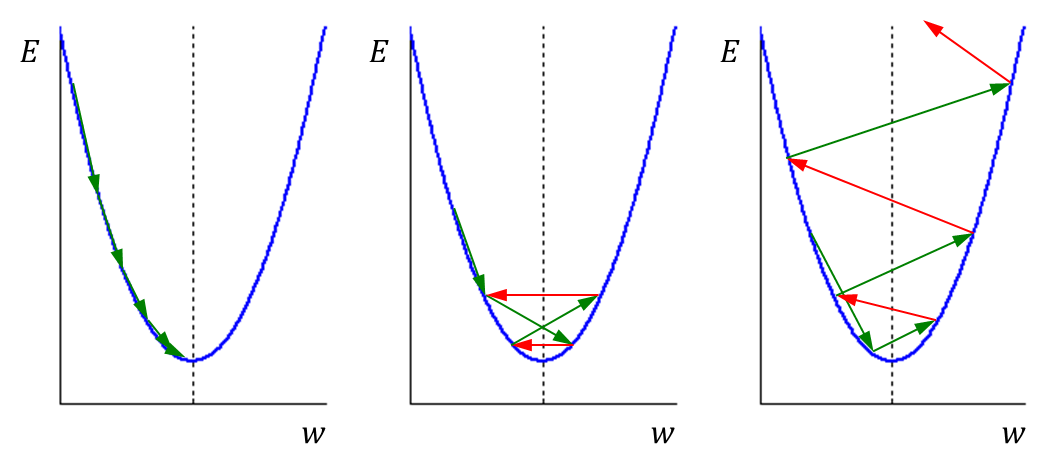
\includegraphics[scale=0.5]{../../pic/bp.png}
        \caption{Possible weight update trends, includes convergence (left), oscillation (middle) and divergence (right).  The solid curve represents error vs. weight, local minimum is at the intersection between the solid curve and the dash line, red arrows represent weight update with positive gradient, and green arrows represent weight update with negative gradient.}
        \label{fig:bp}
	\end{centering}
\end{figure}

To avoid complicate choices among learning rates, some local adaptive learning algorithms have been developed.

\subsection{Quick Propagation (QP)}

The target of quick-propagation is to take the largest steps possible to local minima without overshooting.  The basic idea is to directly jump to a local minimum closely enough.  Risky assumption is made as the error versus weight curve for each weight can be approximated by a parabola whose arms open upward \cite{fahlman1988empirical}, which means its second derivative is approximate a line with positive $k$.  For a parabola curve, the minimum value is where its second derivative equals to 0.

\begin{figure}[tb]
    \begin{centering}
        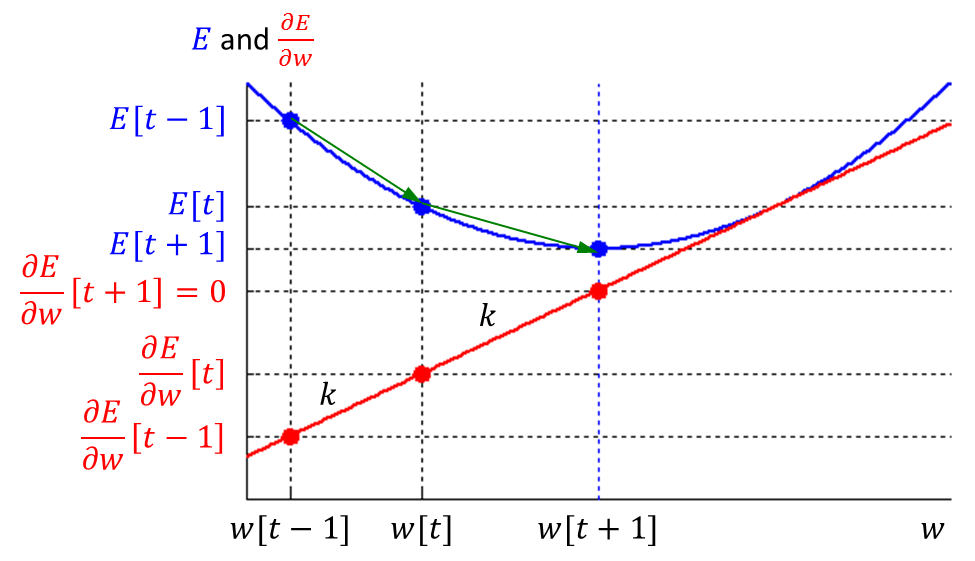
\includegraphics[scale=0.5]{../../pic/qp.png}
        \caption{Gradient (blue solid parabola) and its first derivative (red solid line).  Minimum error is reached at which the first derivative equals to zero.}
        \label{fig:qp}
	\end{centering}
\end{figure}

\begin{gather}
    k = \frac{ \frac{ \partial E }{ \partial w } [ t - 1 ] - \frac{ \partial E }{ \partial w } [t] }{ w[ t - 1 ] - w[t] } = \frac{ \frac{ \partial E }{ \partial w } [t] - 0 }{ w[t] - w[ t + 1 ] } \notag \\
    \Delta w[t] = \frac{ \frac{ \partial E }{ \partial w } [t] }{ \frac{ \partial E }{ \partial w } [ t - 1 ] - \frac{ \partial E }{ \partial w } [t] } \cdot \Delta w[ t - 1 ] \notag \\
    w[ t + 1 ] = w[t] + \Delta w[t] \notag
\end{gather}

According to above equation, if $\frac{ \partial E }{ \partial w } [ t - 1 ]$ is approximate the same as $\frac{ \partial E }{ \partial w } [t]$, $\Delta w[t]$ will reach an infinite value, which leads to an infinite step or towards a local maximum.  To restrain weight change, a maximum growth factor $\mu$is defined in order that no weight step is allowed to be greater in magnitude than μ times the previous step.  A fit-to-all value of $\mu = 1.75$ \cite{fahlman1988empirical}.

\subsection{Resilient Propagation (RP)}

The basic idea of resilient propagation is that every time the gradient changes its sign, which indicates the last update was so big that jumped over a local minimum.  Thus, the weight update absolute value $\theta$ needs to be reduced by factor $\eta ^ -$, where $0 < \eta ^ - < 1$.  Contrarily, if the gradient remains the same sign as previous, a larger step of $\theta$ can be increased by factor $\eta ^ +$, where $\eta ^ + > 1$.  The algorithm can be implemented in following approach \cite{riedmiller1993direct}.
\newline

\indent
for all weights of neurons and bias,

\indent
\{

\indent \indent
if \( \frac{ \partial E }{ \partial w } [ t - 1 ] \cdot \frac{ \partial E }{ \partial w } [t] > 0 \)

\indent \indent
\{

\indent \indent \indent
\( \theta[t] = \eta ^ + \theta[ t - 1 ] \)

\indent \indent \indent
\( \Delta w[t] = - \theta[t] \cdot sign \left( \frac{ \partial E }{ \partial w } [t] \right) \)

\indent \indent
\}

\indent \indent
else if \( \frac{ \partial E }{ \partial w } [ t - 1 ] \cdot \frac{ \partial E }{ \partial w } [t] < 0 \)

\indent \indent
\{

\indent \indent \indent
\( \theta[t] = \eta ^ - \theta[ t - 1 ] \)

\indent \indent \indent
\( \Delta w[t] = - \Delta w[ t - 1 ] \)

\indent \indent \indent
\( \frac{ \partial E }{ \partial w } [t] = 0 \)

\indent \indent
\}

\indent \indent
else

\indent \indent
\{

\indent \indent \indent
\( \Delta w[t] = - \theta[t] \cdot sign \left( \frac{ \partial E }{ \partial w } [t] \right) \)

\indent \indent
\}


\indent \indent
\( w[ t + 1 ] = w[t] + \Delta w[t] \)

\indent \indent
store current \(t\) state variables to next epoch.

\indent
\}
\newline

Intuitively, the algorithm makes it confident for the weights updated to reach local minima.

\begin{figure}[h]
    \begin{centering}
        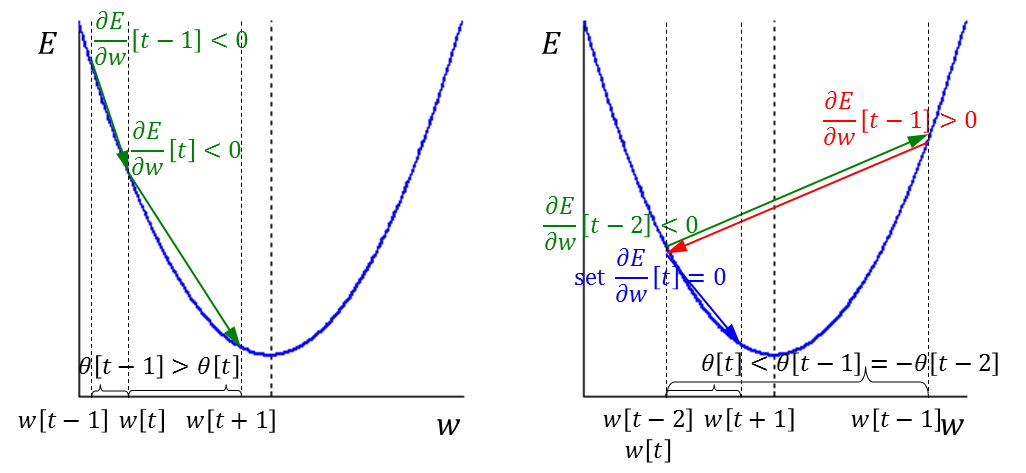
\includegraphics[scale=0.5]{../../pic/rp.png}
        \caption{When gradient doesn’t change its sign (left), weight takes a larger step by a ratio $\eta ^ + > 1$ to update.  When gradient changes its sign (right), weight doesn’t update at this epoch but will take a smaller step by a ratio $0 < \eta ^ - < 1$ to update at next epoch.}
        \label{fig:rp}
	\end{centering}
\end{figure}

Concluded after some experiments \cite{riedmiller1993direct}, slight variation of $\eta ^ -$ or $\eta ^ +$ will neither improve nor deteriorate convergence time.  These two factors are fixed to $\eta ^ - = 0.5$ and $\eta ^ + = 1.2$.  As a similar consequence, the initial values of all $\theta$ are set to 0.1.

\subsection{Levenberg-Marquardt Algorithm (LM)}

Mathematically, Levenberg-Marquardt algorithm aims at solving out non-linear least square problem.  It is much more efficient than other techniques applied to a neural network no more than hundreds of weights, even if the computation requirements are higher than other algorithms within iterations \cite{hagan1994training}.

Gauss-Newton’s method gives out an update to the weight,

\begin{equation}
    \Delta \mathbf{w} = - [ \nabla ^ 2 f( \mathbf{w} ) ] ^ {-1} \nabla f( \mathbf{w} ) \notag
\end{equation}

where $\nabla ^ 2 f( \mathbf{w} )$ is the Hessian matrix and $\nabla f( \mathbf{w} )$ is the gradient.  The Hessian matrix can be approximated by,

\begin{equation}
    \nabla ^ 2 f( \mathbf{w} ) \approx \mathbf{J} ^ \top ( \mathbf{w} ) \mathbf{J} ( \mathbf{w} ) ) \notag
\end{equation}

and the gradient vector can be calculated as,

\begin{equation}
    \nabla f( \mathbf{w} ) = \mathbf{J} ^ \top ( \mathbf{w} ) \mathbf{e} ( \mathbf{w} ) = \mathbf{J} ^ \top ( \mathbf{w} ) [ \mathbf{T} - f( \mathbf{w} ) ] \notag
\end{equation}

where $\mathbf{J}( \mathbf{w} )$ is the Jacobian matrix with $M$ as the network output number and $N$ as the weight number connected to a single neuron.

\begin{equation}
    \mathbf{J}( \mathbf{w} ) =
    \begin{bmatrix}
        \frac{ \partial e_1( \mathbf{w} ) }{ \partial w_1 } & \frac{ \partial e_1( \mathbf{w} ) }{ \partial w_2 } & \cdots & \frac{ \partial e_1( \mathbf{w} ) }{ \partial w_N } \\
        \frac{ \partial e_2( \mathbf{w} ) }{ \partial w_1 } & \frac{ \partial e_2( \mathbf{w} ) }{ \partial w_2 } & \cdots & \frac{ \partial e_2( \mathbf{w} ) }{ \partial w_N } \\
        \vdots & \vdots & \ddots & \vdots \\
        \frac{ \partial e_M( \mathbf{w} ) }{ \partial w_1 } & \frac{ \partial e_M( \mathbf{w} ) }{ \partial w_2 } & \cdots & \frac{ \partial e_M( \mathbf{w} ) }{ \partial w_N }
    \end{bmatrix} \notag
\end{equation}

Thus, the Gauss-Newton’s method updates weights as,

\begin{equation}
    \Delta \mathbf{w} = [ \mathbf{J} ^ \top ( \mathbf{w} ) \mathbf{J} ( \mathbf{w} ) ] ^ {-1} [ \mathbf{J} ^ \top ( \mathbf{w} ) \mathbf{e} ( \mathbf{w} ) ] \notag
\end{equation}

Levenberg-Marquardt algorithm modifies above equation to ensure the inversion of matrix always exists by,

\begin{equation}
    \Delta \mathbf{w} = [ \mathbf{J} ^ \top ( \mathbf{w} ) \mathbf{J} ( \mathbf{w} ) + \lambda \mathbf{I} ] ^ {-1} [ \mathbf{J} ^ \top ( \mathbf{w} ) \mathbf{e} ( \mathbf{w} ) ] \notag
\end{equation}

where $\lambda$ is a changeable damping parameter.  $\lambda$ will increase if squared error $E = \mathbf{e} ^ \top ( \mathbf{w} ) \mathbf{e} ( \mathbf{w} )$ increases, $\lambda$ will decrease if squared error reduced, that is,

\begin{equation}
    \lambda [t] = \left \{
    \begin{array}{l l}
        \beta \lambda [ t - 1 ] & \quad E[t] > E[ t - 1 ] \\
        \frac{1}{\beta} \lambda [ t - 1 ] & \quad E[t] < E[ t - 1 ]
    \end{array} \right. \notag
\end{equation}

A good try for initial value of $\lambda$ could be 0.01 and the factor $\beta > 1$ could be 10.  In addition, if squared error increase, weight will be reverted to previous value.

%------------------------------------------------------------------------------

\section{Performance and Experiment Result}

Briefly sum up previous techniques, this library implements four back-propagation algorithms, parallelization, abstraction and generalization.  In order to evaluate the performance of such techniques, several experiments have been conducted by controlling variables.  All following experiments are running on a 2.3GHz quad-core 8-thread CPU with 8G RAM machine installing 64-bit operating system.

Experiment data is selected from hourly historical climate data of Ann Arbor, MI, USA downloaded from \url{www.wunderground.com} from year 2010 to 2013, year 2010 to 2012 as training samples and year 2013 as testing samples.  So total number of training samples is 26304, total number testing samples is 8760.  Training samples are averagely distributed on each thread of which the number is determined by the configuration of each experiment.  10 input features listed in table~\ref{table:climate} are fed into each experiment system and the humidity value is the only one output.  All of them are normalized to zero mean ($\mu = 0$) and unit standard derivation ($\sigma = 1$).

\begin{table}[htp]
    \centering
    \caption{Features in climate dataset}
    \begin{tabular}{ c l c c }
        \hline \hline
        Usage & Feature & Valid Range & Unit \\
        \hline
        \multirow{10}{*}{input}
            & month & 1 - 12 & - \\
            & hour & 0 - 23 & - \\
            & temperature & -50 - 150 & \(^\circ\)F \\
            & dew point & -50 - 150 & \(^\circ\)F \\
            & pressure & 28 - 31 & inHg \\
            & visibility & 0 - 10 & mile \\
            & wind direction & 0 - 359 & \(^\circ\) \\
            & wind speed & 0 - 50 & mph \\
            & gust speed & 0 - 100 & mph \\
            & precipitation & 0 - 1.5 & in \\
        \hline
        target & humidity & 0 - 100 & \% \\
        \hline \hline
    \end{tabular}
    \label{table:climate}
\end{table}

\subsection{Multithread Efficiency}

Theoretically, multiple processors and cores can simulate almost any number of threads running simultaneously regardless of very large system specified limit.  However, the communication between threads is usually implemented by a pooling approach.  As a result, it will consume certain amount of time to synchronize all the image threads to main network thread.  Intuitively, the most efficient number of threads should be equal to the number of cores, since running time of multithreads on the same core will add up to no less than the running time of single thread even though any kind of thread scheduling applied.

Here is the experiment result using the same network configuration as shown in table~\ref{table:config_thread_efficiency} and same amount of data but different numbers of threads doubled from 1 to $2 ^ N$.  BP algorithm is used in this experiment, maximum epoch is set to 2000 and algorithm coefficients will not affect the execution time.

\begin{table}[htp]
    \centering
    \caption{Training time for different hidden node number using different thread number}
    \begin{tabular}{ c c | c c c c c }
        \hline \hline
            \multicolumn{2}{ c | }{ \multirow{2}{*}{ training time (s) } }
          & \multicolumn{5}{c}{hidden node number} \\
          && 10 & 20 & 20 & 40 & 50 \\
        \hline
        \multirow{10}{*}{thread number (\( 2 ^ N \))}
            & 1 & 132 & 428 & 850 & 1390 & 2148 \\
            & 2 & 80 & 269 & 539 & 883 & 1373 \\
            & 4 & 62 & 212 & 420 & 693 & 1045 \\
            & 8 & 46 & 161 & 311 & 576 & 953 \\
            & 16 & 49 & 163 & 316 & 614 & 973 \\
            & 32 & 50 & 165 & 313 & 590 & 965 \\
            & 64 & 53 & 165 & 315 & 595 & 976 \\
            & 128 & 59 & 172 & 323 & 608 & 975 \\
            & 256 & 75 & 186 & 344 & 630 & 1018 \\
            & 512 & 119 & 214 & 381 & 676 & 1054 \\
        \hline \hline
    \end{tabular}
    \label{table:thread_efficiency}
\end{table}

\begin{figure}[tb]
    \centering
    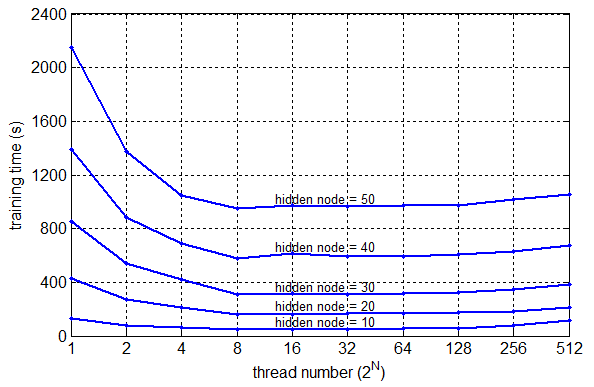
\includegraphics[scale=0.6]{../../pic/efficiency.png}
    \caption{Training time for different hidden node number configuration versus different numbers of threads.  Curves from bottom to top corresponding to the network hidden node number equals to 10, 20, 30, 40 and 50.}
    \label{fig:thread_efficiency}
\end{figure}

The result demonstrates that the fastest thread configuration number start from 8, which equals to the thread number and hardware concurrency of CPU in this case.  It is about 3-time ($\frac{132}{46} \approx 2.87$) faster than training with single thread training a 10 hidden nodes network, but it is not able to reach an ideal 8-time because of communication problem mentioned before.  With the increase number of threads more than 8, training time slightly goes up because of scheduling problem mentioned before.

\begin{table}[htp]
    \centering
    \caption{Neural network configuration for multithread efficiency experiment}
    \begin{tabular}{ l l }
        \hline \hline
        Affected Parameter & Configuration \\
        \hline
        input node number & 10 \\
        hidden layer number & 2 \\
        hidden node number & 10, 20, ..., 50 \\
        hidden layer transfer function & log-sigmoid \\
        output node number & 1 \\
        output layer transfer function & linear \\
        neural learning algorithm & BP \\
        stop early & no \\
        \hline \hline
    \end{tabular}
    \label{table:config_thread_efficiency}
\end{table}

\subsection{Algorithm Complexity}

For the same network structure, different algorithm will take various number of CPU instructions to execute, thus it greatly affect training time among different algorithms.  In this experiment, maximum epoch is set to 2000 and algorithm coefficients in table~\ref{table:config_algorithm_complexity} will not affect the execution time.  A baseline is set under the help of Matlab Neural Networks Toolbox with the same network parameters set.  Another 10 measurements are taken independently from previous experiment, mean values are presented and standard deviation is presented as reliability.

\begin{table}[htp]
    \centering
    \caption{Training time at different thread number}
    \begin{tabular}{ l c c c c }
        \hline \hline
        Traing Time (s) & BP & QP & RP & LM \\
        \hline
        8-thread GPNN & 56.8 & 69.7 & 62.4 & 263.9 \\
        1-thread GPNN & 176.7 & 192.3 & 167.9 & 337.7 \\
        1-thread Matlab & 649.1 & 678.1 & - & 1264.0 \\
        \hline \hline
    \end{tabular}
    \label{table:algorithm_complexity}
\end{table}

Results in table~\ref{table:algorithm_complexity} show that the LM algorithm takes far more time to be trained than other algorithms.  This is because Hessian matrix inversion needs to be calculated frequently even during each iteration \cite{yu2011levenberg}.  The speed is gained by second-order approximation to the number of weights.  Multithread technique does not accelerate the training process of LM algorithm because the time consumption of communication among threads is now a less distinct factor compared to that of matrix inversion.

\begin{table}[htp]
    \centering
    \caption{Neural network configuration for algorithm complexity experiment}
    \begin{tabular}{ l l }
        \hline \hline
        Affected Parameter & Configuration \\
        \hline
        thread number & 1 and 8 \\
        neural learning algorithm & BP, QP, RP and LM \\
        \multicolumn{2}{c}{Other parameters are the same as in table \ref{table:config_thread_efficiency}.} \\
        \hline \hline
    \end{tabular}
    \label{table:config_algorithm_complexity}
\end{table}

\subsection{Algorithm Efficiency}

In reality, it is unnecessary to complete a training process up to specified maximum epoch.  Training could be terminated if certain criteria meet, for example, sum of error or gradient approximates to 0, gradient doesn’t distinctly decrease for several epochs.  Training time, converge epochs, converge error and at the termination are three measurements of efficiency among different back-propagation algorithms.  All developed algorithms participate in the comparison experiment here as configured in table~\ref{table:config_algorithm_efficiency}.  As soon as the mean absolute value of gradient is less than $10 ^ {-9}$ or not changing for 6 epochs \cite{matlab:neural_networks}, training will stop which means that error converges.  Another 10 measurements are taken independently from previous experiments and the average values are presented and standard deviation is presented as reliability.

\begin{table}[htp]
    \centering
    \caption{Converge epochs and errors of different algorithms}
    \begin{tabular}{ l c c c c }
        \hline \hline
        & BP & QP & RP & LM \\
        \hline
        training time (s) & 3.5 & 35.1 & 28.2 & 31.1 \\
        converge epoch & 43.2 & 976.4 & 866.7 & 97.2 \\
        training error (\%) & 3.80 & 1.86 & 0.73 & 3.15 \\
        testing error (\%) & 3.66 & 1.88 & 0.76 & 33.08 \\
        \hline \hline
    \end{tabular}
    \label{table:algorithm_efficiency}
\end{table}

Results in table~\ref{table:algorithm_efficiency} shows that LM converges faster than QP and RP, especially LM.  However, it takes relatively more time to run because of matrix inversion time consumption discussed before.  Although RP takes more epochs to converge, its training and testing errors are distinctly smaller than others’.

According to this experiment and under the application scenario, if high accuracy is required for prediction or classification, RP algorithm is a good fit to deep dig out the local minima.  If big dataset applied and there’s no specific accuracy requirement, BP and QP algorithm could be applied.  If no more than hundreds of hidden nodes are needed, LM could be efficient as well.

\begin{table}[htp]
    \centering
    \caption{Neural network configuration for algorithm efficiency experiment}
    \begin{tabular}{ c c c c c }
        \hline \hline
        & BP & QP & RP & LM \\
        \hline
        thread number & 8 & 8 & 8 & 8 \\
        $\eta$ & 0.5 & 0.5 & - & - \\
        $\mu$ & - & 1.75 & - & - \\
        $\eta ^ -$ & - & - & 0.5 & - \\
        $\eta ^ +$ & - & - & 1.2 & - \\
        $\theta$ & - & - & 0.1 & - \\
        \hline \hline
    \end{tabular}
    \label{table:config_algorithm_efficiency}
\end{table}

%------------------------------------------------------------------------------

\section{Conclusion}

Based on the architecture and design pattern of this neural networks library, the author developed multiple weight update algorithms one by one after reviewing different back-propagation techniques without greatly modifying other components inside the architecture.  In terms of this, the library could be regarded as easily extendable, especially facing the circumstance that future algorithms being developed continuously.

The author created this library under the consideration of both abstraction and generalization.  It produces benefits if a network structure is not symmetric, which means user can customize the topology by pruning or branching the connections during programming.

The multithreaded architecture could easily be embedded into any kind of distributed systems by calling few functions the library provides.

The Multithreaded Neural Networks Template Library GPNN under LGPL license is available at
\url{github.com/wenduow/BeefNet}

%------------------------------------------------------------------------------

\appendix

%------------------------------------------------------------------------------

\section{Comparison with Other Neural Networks Library}
\label{appendix:comparison}



\begin{table}[htp]
    \centering
    \caption{Neural network library characteristics}
    \begin{tabular}{ >{\centering}m{3cm} c c c c }
        \hline \hline
        Supports & FANN & OpenNN & tnnlib & GPNN \\
        \hline
        parallel computing interface & N & N & N & Y \\
        \hline 
        neural learning algorithm diversity & Y & Y & Y & Y \\
        \hline
        generic programming (strong scalability) & N & N & Y & Y \\
        \hline \hline
    \end{tabular}
    \label{table:library_compare}
\end{table}

%% References with BibTeX database:

\bibliographystyle{plain}
\bibliography{my_ref}

\end{document}

% EOF

